\documentclass[a4paper,11pt]{article}

\usepackage{mathpazo}
\usepackage{url}
\usepackage{tikz}
\usetikzlibrary{through,calc,intersections}
\tikzset{>=stealth}
\newcommand*{\vertex}[1]
  {\fill[shift only] (#1) circle (1.5pt)}
\newcommand*{\sm}[1]{$\scriptstyle #1$}
\newcommand*{\disfrac}[2]{\displaystyle\frac{#1}{#2}}

% Layout
\textwidth=145mm
\textheight=230mm
\topmargin=0pt
\headheight=0pt
\oddsidemargin=10mm
\evensidemargin=0mm
\headsep=0pt
\parindent=0pt
\renewcommand{\baselinestretch}{1.1}
\setlength{\parskip}{0.3\baselineskip plus 1pt minus 1pt}


\newcommand\qed{\hfill\hbox{\rlap{$\sqcap$}$\sqcup$}}
\newtheorem{theorem}{Theorem}
\newenvironment{proof}{\textbf{Proof}}{\qed}
\addtolength{\arraycolsep}{-3pt}

%%%%%%%%%%%%%%%%%%%%%%%%%%%%%%%%%%%%%%%%%%%%%%%%%%%%%%%%

\begin{document}

\begin{center}
\bfseries\Large
A Regular Heptadecagon is Constructible

\medskip

Moti Ben-Ari
\end{center}

\textbf{Introduction}

For centuries people learned mathematics by studying Euclid's \textit{Elements}. A focus of the \textit{Elements} is on the construction of geometric figures using a straightedge (a ruler with no markings) and a compass. The \textit{Elements} gives constructions of regular polygons with $n=3,4,5,15$ sides (and polygons with $2^kn$ sides), but not until two thousand years later was the construction of another regular polygon discovered. In $1796$ Carl Friedrich Gauss awoke one morning just before his 19th birthday, and by ``concentrated thought'' discovered that a regular heptadecagon (a regular polygon with $17$ sides) is constructible. It was a  revolutionary development because Gauss proved the constructibility \emph{algebraically} not geometrically.

\textbf{Constructibility}

The first proposition in the \textit{Elements} is that an equilateral triangle can be constructed. (The word ``construct'' will be used as an abbreviation for ``construct by straightedge and compass.'') Given a line segment $\overline{AB}$ draw two circles whose centers are $A,B$ and whose radii are the length of $\overline{AB}$. $C$, the intersection of the circles, defines the third vertex of the triangle:
\begin{center}
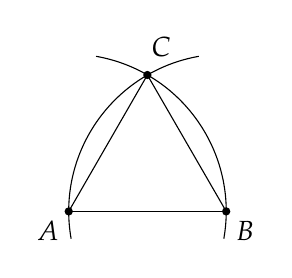
\begin{tikzpicture}[scale=0.5]
\coordinate (A) at (0,0);
\coordinate (B) at (4,0);
\draw (A) node[below left] {$A$} -- (B) node[below right] {$B$};
\vertex{A};
\vertex{B};
\draw[name path=larc] (A) ++(-10:4cm) arc (-10:80:4cm);
\draw[name path=rarc] (B) ++(190:4cm) arc (190:100:4cm);
\path [name intersections={of=larc and rarc,by={t}}];
\vertex{t};
\node[above right,xshift=-2pt,yshift=3pt] at (t) {$C$};
\draw (A) -- (t) -- (B);
\end{tikzpicture}
\end{center}

Define a real number $x$ to be \textit{constructible} if and only if starting with a line segment defined to be of length $1$ it is possible to construct a line segment of length $x$.

\textbf{Theorem:} $x$ is constructible if and only if it is the result of evaluating an expression composed from the integer $1$ using the operations $\{+,-,\times,/,\surd\}$.

Here is an outline of the proof:
\begin{itemize}
\item Lines are defined by linear equations and circles by quadratic equations, so the intersections of lines and circles are the solutions of two such equations. Expressions for the coordinates of the intersections (and hence the length of line segments between two points) must also be composed from integers and the operations $\{+,-,\times,/,\surd\}$.
\item Given two line segments, their sum and difference can be obtained by copying one onto the other or onto an extension of the other. The following diagrams show how to construct products, differences and square roots using similar triangles.
\end{itemize}
\begin{center}
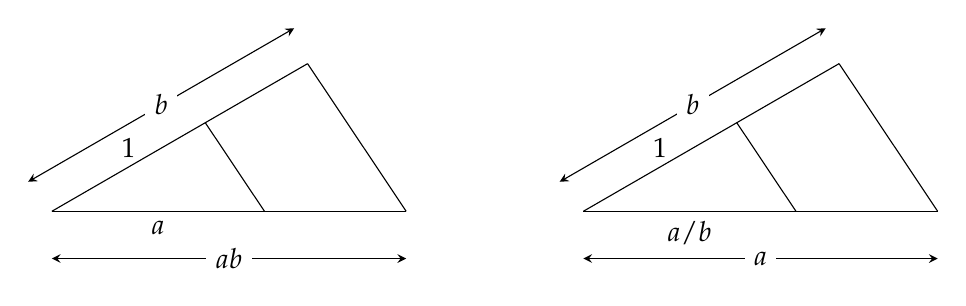
\begin{tikzpicture}[scale=.75]
\draw[name path=horz] (0,0) coordinate (o) -- (6,0);
%\node[left] at (o) {$O$};
\coordinate (a) at (6,0);
%\node[below]  at (a) {$A$};
\draw (o) -- (30:5);
\coordinate (c) at (30:3);
\coordinate (b) at (30:5);
%\node[above] at (c) {$C$};
%\node[above] at (b) {$B$};
\draw (a) -- (b);
\path[name path=par] (c) -- +($(a)-(b)$);
\path[name intersections={of=par and horz,by=d}];
%\node[below] at (d) {$D$};
\draw (c) -- (d);
\draw[<->] (-.4,.5) -- node[fill=white] {$b$} +(30:5.2);
\path (o) -- node[above] {$1$} (c);
\draw[<->] (0,-.8) -- node[fill=white] {$ab$} +(6,0);
\path (o) -- node[below] {$a$} (d);
\begin{scope}[xshift=9cm]
\draw[name path=horz] (0,0) coordinate (o) -- (6,0);
%\node[left] at (o) {$O$};
\coordinate (a) at (6,0);
%\node[below]  at (a) {$A$};
\draw (o) -- (30:5);
\coordinate (c) at (30:3);
\coordinate (b) at (30:5);
%\node[above] at (c) {$C$};
%\node[above] at (b) {$B$};
\draw (a) -- (b);
\path[name path=par] (c) -- +($(a)-(b)$);
\path[name intersections={of=par and horz,by=d}];
%\node[below] at (d) {$D$};
\draw (c) -- (d);
\draw[<->] (-.4,.5) -- node[fill=white] {$b$} +(30:5.2);
\path (o) -- node[above] {$1$} (c);
\draw[<->] (0,-.8) -- node[fill=white] {$a$} +(6,0);
\path (o) -- node[below] {$a/b$} (d);
\end{scope}
\end{tikzpicture}
\end{center}
\begin{center}
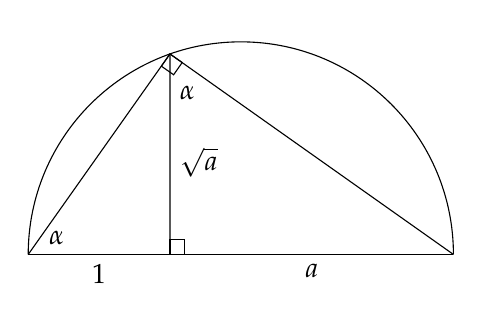
\begin{tikzpicture}[scale=.9]
\draw[name path=horz] (0,0) coordinate (a) -- (6,0);
%\node[left] at (a) {$A$};
\coordinate (b) at (6,0);
%\node[below] at (b) {$B$};
\draw[name path=circle] (b) arc(0:180:3);
\path[name path=perp] (2,0) -- +(0,3.2);
\coordinate (c) at (2,0);
%\node[below] at (c) {$C$};
\path[name intersections={of=circle and perp,by=d}];
%\node[above] at (d) {$D$};
\draw (c) -- node[right,yshift=-3pt] {$\sqrt{a}$} (d);
\path (a) -- node[below] {$1$} (c) -- node[below] {$a$} (b);
\draw (c) rectangle +(6pt,6pt);
\draw (a) -- (d) -- (b);
\draw[rotate=-125] (d) rectangle +(6pt,6pt);
\node[above right,xshift=4pt] at (a) {$\alpha$};
%\node[above left,xshift=-12pt] at (b) {$90^\circ-\alpha$};
\node[below right,yshift=-8pt] at (d) {$\alpha$};
%\node[below left,xshift=3pt,yshift=-22pt] at (d) {$90^\circ-\alpha$};
\end{tikzpicture}
\end{center}

\textbf{Impossible constructions}

The Greeks were unable to trisect an angle (divide a given angle into three equal parts), square a circle (construct a square with the same area as a given circle) and double a cube (construct a cube with twice the volume of a given cube). During the nineteenth century it was proved that these constructions are impossible. Of equal interest was the construction of regular polygons. The Greeks were unable to construct regular polygons with $n=7,9,11,13,14,17,18,\ldots$ sides.

\textbf{The mathematics of constructibility}

A regular polygon can be inscribed in a unit circle. The polygon can be constructed if and only the central angle subtended by one of its sides (or the cosine of the angle) can be constructed. In the following diagram $\overline{AC}$ is a side of the polygon.
\begin{center}
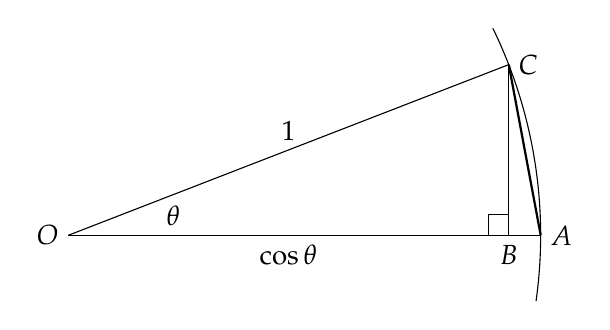
\begin{tikzpicture}[scale=1.5]
\coordinate (O) at (0,0) node[left] {$O$} node[above right,xshift=32pt] {$\theta$};
\coordinate (A) at (4,0);
\node[right] at (A) {$A$};
\draw (O) -- (A);
\draw (-8:4) arc (-8:26:4);
%\draw (A) arc(0:21.18:4);
\coordinate (C) at (21.18:4cm);
\draw (O) -- node[above] {$1$} (C);
\node[right] at (C) {$C$};
\draw (C) -- (C |- A) coordinate (B);
\node[below] at (B) {$B$};
\draw[rotate=90] (B) rectangle +(5pt,5pt);
\draw[thick] (A) -- (C);
\path (O) -- node[below] {$\cos \theta$} (B); 
\end{tikzpicture}
\end{center}
The central angle of an equilateral triangle is $120^\circ$ and $\cos 120^\circ=-1/2$ is constructible. The central angle of a regular pentagon is $72^\circ$ and it is not too hard to show that $\cos 72^{\circ}=(\sqrt{5}-1)/4$, so a regular pentagon is constructible. A regular pentadecagon (a regular polygon with $15$ sides) is constructible since its central angle is $360^\circ/15=24^\circ=(120^\circ-72^\circ)/2$. We want to show that the angle $360^\circ/17$ or its cosine is constructible.

\textbf{Mathematical prerequisites}

With one exception we will only use secondary-school algebra: multiplication of variables with exponents,
% $x^nx^m=x^{n+m}$, 
integer division with remainder,
%$a=bq+r, 0\leq r < q$, 
and finding the roots of quadratic equations.
% $x^2+bx+c$ from the formula $r_1,r_2=(-b\pm\sqrt{b^2-4c})/2$. 
The exception is the Fundamental Theorem of Algebra, which states that an $n$-th degree polynomial with complex coefficients has $n$ complex roots. Actually, we only need one simple case of the theorem: the polynomial $x^{n}-1$ has (at least) one root $r\neq 1$ or, even more narrowly, that $x^{17}-1$ has (at least) one root $r\neq 1$

%In terms of complex numbers, the root is $r=\cos \left(\frac{2\pi}{n}\right) + i\sin  \left(\frac{2\pi}{n}\right)$, since by de Moivre's formula:
%\[
%\left[\cos \left(\frac{2\pi}{n}\right) + i\sin  \left(\frac{2\pi}{n}\right)\right]^{n}=
%\cos \left(\frac{2 n\pi}{n}\right) + i\sin  \left(\frac{2 n\pi}{n}\right)= 1\,.
%\]
%However, this is not necessary for the proof since we are searching for an expression that is constructible.
%

\textbf{The roots of unity}

The roots of $x^{n}-1$ are called the \emph{$n$-th roots of unity}. If $r$ is an $n$-th root of unity then $(r^{2})^n=(r^{n})^2=1^2=1$ so $r^2$ is also an $n$-th root of unity. It follows that $1, r, r^2, \ldots, r^{n-2}, r^{n-1}$ are all $n$-th roots of unity. What we don't know is if they are distinct and thus all the $n$-th roots of unity. For example, the roots of the polynomial $x^4-1$ are $1,-1,i,-i$, but $(-1)^2=1$, $(-1)^3=-1$, $(-1)^4=1$ so the powers of $r=-1$ are not distinct and do not give all the fourth roots of unity.

\textbf{Theorem:} If $n$ is a prime number and $r$ is an $n$-the root of unity then $1,r,r^2,\ldots,r^{n-2},r^{n-1}$ are distinct.

\textbf{Proof:} If $r^i=r^j$ for some $0\leq i<j\leq n-1$ then $r^j/r^i=r^{j-i}=1$. Let $m$ be the smallest positive integer such that $r^{m}=1$. By the division formula:
\[
1=r^n=r^{ml+k}=(r^m)^l\cdot r^k=1^l\cdot r^k=r^k\,,
\]
where $0\leq k<m$, but $0<k$ and $r^k=1$ contradict the assumption that $m$ was the smallest such positive number. Therefore, $k=0$ and $n=ml$ is not prime.

\textbf{From roots back to coefficients of polynomials}

Suppose that we know the values of $r_1,r_2$, two roots of a quadratic polynomial $x^2+bx+c$. What are the coefficients? By computation:
\[
(x-r_1)(x-r_2)=x^2 - (r_1+r_2)x + r_1r_2=x^2+bx+c\,,
\]
so
\begin{equation}\label{eq.v1}
b=-(r_1+r_2), \qquad c=r_1r_2\,,
\end{equation}
and similarly the coefficients of any polynomial can be computed if the roots are known. Given that the roots of $x^{17}-1$ are $\{1,r,r^2,\cdots, r^{15}, r^{16}\}$, we can find and coefficient of the polynomial by multiplying $(x-1)(x-r^1)(x-r^2)\cdots (x-r^{15})(x-r^{16})$. The coefficient of $x^{16}$ is:
\[
-(1+r^1+r^2+\cdots+r^{15}+r^{16})\,,
\]
which is $0$ in $x^{17}-1$ so:
\begin{equation}\label{eq.sum-is-minus1}
r^1+r^2+\cdots+r^{15}+r^{16}=-1\,.
\end{equation}

\textbf{Gauss's proof that the heptadecagon is constructible}

Gauss's insight was that we need not work with the roots in their natural order $r,\cdots,r^{16}$, but that other powers of roots can generate all the roots. Starting from $r$, repeatedly raising it to the third power (modulo $17$) gives:
\[
\begin{array}{l}
r^1, \;(r^1)^3 =r^3,\; (r^3)^3=r^9,\; (r^9)^3=r^{27}=r^{10}, \; (r^{10})^3=r^{30}=r^{13}, \;\ldots \,.
\end{array}
\]
The reader is invited to compute the roots and check that the following list contains all the roots (except $1$) exactly once:
\[
\begin{array}{rrrrrrrrrrrrrrrr}
r^1& r^3& r^9& r^{10}& r^{13}& r^5& r^{15}& r^{11}& r^{16}& r^{14}& r^8& r^7& r^4& r^{12}& r^2& r^6\,.
\end{array}
\]
Write the roots as follows in order to emphasize the roots in the odd and even positions:
\[
\begin{array}{rrrrrrrrrrrrrrrr}
r^1 &&  r^9 &&  r^{13} && r^{15} &&  r^{16} && r^8 && r^4 && r^2\\\
&r^3&& r^{10}&& r^5&& r^{11}&& r^{14} &&  r^7&& r^{12}&& r^6\,.
\end{array}
\]
Let $a_0, a_1$ be the sums of the roots in the odd and even positions, respectively:
\begin{eqnarray*}
a_0&=&r + r^9 + r^{13} +r^{15} +r^{16} + r^8+r^4+r^2\\
a_1&=&r^3 + r^{10} + r^{5} +r^{11} +r^{14} + r^7+r^{12}+r^6\,.
\end{eqnarray*}
Compute $a_0+a_1$ using Equation~\ref{eq.sum-is-minus1}:
\[
a_0+a_1=r + r^2 + \cdots +r^{16}=-1\,.
\]
Now compute $a_0a_1$ and simplify. It takes quite a lot of work, but the result is the sum of four copies of Equation~\ref{eq.sum-is-minus1} so:
\[
a_0a_1=-4\,.
\]
Given that $a_0,a_1$ are roots, by Equation~\ref{eq.v1} they are the roots of the polynomial:
\[
y^2+y-4=0\,,
\]
and their values are:
\[
a_0, a_1 = \frac{-1\pm\sqrt{17}}{2}\,.
\]
Let $b_0,b_1,b_2,b_3$ be the sums of every fourth root starting from $r^1,r^3,r^9,r^{10}$, respectively:
\begin{eqnarray*}
b_0&=& r^1+ r^{13} + r^{16} + r^4\\
b_1&=& r^3+ r^{5} + r^{14} + r^{12}\\
b_2&=& r^9+ r^{15} + r^{8} + r^2\\
b_3&=& r^{10}+ r^{11} + r^{7} + r^6\,.
\end{eqnarray*}
Check that $b_0+b_2=a_0, b_1+b_3=a_1$ and compute the corresponding products which are $b_0b_2=b_1b_3=-1$.
%\begin{eqnarray*}
%b_0b_2&=&(r + r^{13} + r^{16} +r^4)\;\;\times\;(r^9 + r^{15} + r^{8} +r^{2})\\
%&=&(r^{10}+r^{16}+r^9+r^3)\,+\;\,(r^{5}+r^{11}+r^4+r^{15})+\\
%&&(r^{8}+r^{14}+r^7+r^1)\,\;\,+\;\,(r^{13}+r^{2}+r^{12}+r^6)\\
%&=&-1\\
%%\end{eqnarray*}
%%
%%\begin{eqnarray*}
%b_1b_3&=&(r^3 + r^{5} + r^{14} +r^{12})\;\;\times\;(r^{10} + r^{11} + r^{7} +r^{6})\\
%&=&(r^{13}+r^{14}+r^{10}+r^9)\;+\;(r^{15}+r^{16}+r^{12}+r^{11})+\\
%&&(r^{7}+r^{8}+r^4+r^3)\quad\;\, +\;(r^{5}+r^{6}+r^{2}+r^1)\\
%&=&-1\,.
%\end{eqnarray*}
%To summarize these computations:
%\begin{eqnarray*}
%b_0+b_2&=&a_0\\
%b_0b_2&=&-1\\
%b_1+b_3&=&a_1\\
%b_1b_3&=&-1\,,
%\end{eqnarray*}
Therefore, $b_0,b_2$ are the solutions of $y^2-a_0y-1= 0$, and $b_1,b_3$ are the solutions of $y^2-a_1y-1 =0$. Using the values previously computed for $a_0,a_1$ we can compute the roots $b_0,b_1$. We will spare the readers the messy algebra and just give the results:
\[
b_0, b_1 =\frac{(-1\pm\sqrt{17}) + \sqrt{34\mp2\sqrt{17}}}{4}\,.
\]
(For $b_0$ take plus and then minus and for $b_1$ take minus and then plus.)

Finally, let $c_0,c_4$ be the sums of every eighth root starting with $r^1,r^{13}$:
\begin{eqnarray*}
c_0&=&r^1+r^{16}\\
c_4&=&r^{13}+r^4\\
c_0+c_4&=&=b_0\\
c_0c_4&=&b_1\,,
%c_0+c_4&=&r^1+r^{16}+r^{13}+r^4=b_0\\
%c_0c_4&=&(r^1+r^{16})\cdot(r^{13}+r^4)\\
%&=&r^{14}+r^5+r^{12}+r^3=b_1\,,
\end{eqnarray*}
so $c_0,c_4$ are the roots of $y^2-b_0y+b_1=0$.

For $\theta=(360^\circ/17)$, $\cos\theta= c_0/2=(r^1+r^{16})/2$:
\begin{center}
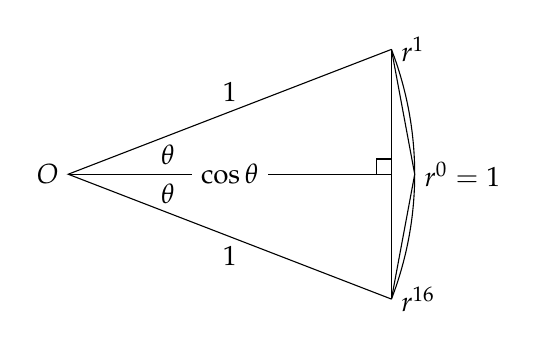
\begin{tikzpicture}[scale=1.1]
\coordinate (O) at (0,0) node[left] {$O$}
  node[above right,xshift=30pt] {$\theta$}
  node[below right,xshift=30pt] {$\theta$};
\coordinate (A) at (4,0);
\node[right] at (A) {$r^0=1$};
\coordinate (C) at (21.12:4cm);
\coordinate (D) at (-21.12:4cm);
\draw (D) arc(-21.12:21.12:4);
\draw (D) -- node[below] {$1$} (O) -- node[above] {$1$} (C);
\node[right] at (C) {$r^1$};
\node[right] at (D) {$r^{16}$};
\draw (C) -- (C |- A) coordinate (B);
\draw (D) -- (D |- A);
\draw[rotate=90] (B) rectangle +(5pt,5pt);
\draw (D) -- (A) -- (C);
\draw (O) --  node[fill=white] {$\cos \theta$} (B);
\end{tikzpicture}
\end{center}
so it suffices to compute the root $c_0$. The result is:
\begin{eqnarray*}
\cos\left(\disfrac{360^\circ}{17}\right) &=& 
\disfrac{c_0}{2}\\
&=&-\disfrac{1}{16}+\disfrac{1}{16}\sqrt{17} + 
     \disfrac{1}{16}\sqrt{34-2\sqrt{17}}\; +\\
 &\;\;& \quad\disfrac{1}{16}\sqrt{
     68+12\sqrt{17} + 
     2(-1+\sqrt{17})\sqrt{34-2\sqrt{17}}
   -16
     \sqrt{34+2\sqrt{17}}
   }\,.
\end{eqnarray*}


The cosine of the central angle of a heptadecagon is constructible since it is the value of an expression composed of integers and the operations $\{+,-,\times,/,\surd\}$!

%With complex numbers it is easy to see the relation between the roots and the cosine of the central angle:
%\begin{eqnarray*}
%r_1+r_{16}&=&\cos\left(\frac{2\pi}{17}\right)+i\sin\left(\frac{2\pi}{17}\right)+\cos\left(\frac{2\cdot 16\pi}{17}\right)+i\sin\left(\frac{2\cdot 16\pi}{17}\right)\\
%&=&\cos\left(\frac{2\pi}{17}\right)+i\sin\left(\frac{2\pi}{17}\right)+\cos\left(\frac{-2\pi}{17}\right)+i\sin\left(\frac{-2\pi}{17}\right)\\
%&=&2\cos\left(\frac{2\pi}{17}\right)\,.
%\end{eqnarray*}
%

The formula that usually appears in the literature is:
\begin{eqnarray*}
\cos\left(\frac{360^\circ}{17}\right)
&=&-\frac{1}{16}+\frac{1}{16}\sqrt{17} + 
     \frac{1}{16}\sqrt{34-2\sqrt{17}}\\
&&+\,\frac{1}{8}\sqrt{
     17+3\sqrt{17} - 
     \sqrt{34-2\sqrt{17}}
   -2
     \sqrt{34+2\sqrt{17}}
   }\,.
\end{eqnarray*}
We leave it to the reader to derive this formula from the one we derived above.

\textbf{Gauss-Wantzel Theorem}

The construction of the regular heptadecagon led to the Gauss-Wantzel theorem, which states that a regular polygon with $n$ sides is constructible if and only if $n$ is the product of a power of $2$ and zero or more \emph{distinct} Fermat numbers $2^{2^k}+1$ which are prime. The known Fermat primes are:
\[
F_0=3,\quad F_1=5,\quad F_2=17,\quad F_3=257,\quad F_4=65537\,.
\]
A regular polygon with $257$ sides was constructed by Magnus Georg Paucker in $1822$ and by Friedrich Julius Richelot $1832$. In $1894$ Johann Gustav Hermes claimed to have constructed a regular polygon  with $65537$ sides.

\textbf{Conclusion}

Until the eighteenth or nineteenth century, mathematical theorems were proved geometrically. Even Newton who invented the calculus used it as a means of discovery and he insisted that a proof must be geometric. This is not surprising since calculus was not placed on a firm theoretical foundation until the late nineteenth century.

Gauss proved the constructibility of the heptadecagon without giving a geometric construction! In fact, the first constructions were not published until almost a century later (a modern construction is given in \cite{callagy}). His algebraic solution led to the growing ascendancy of algebra during the nineteenth century.

%, as indicated by the proliferation of fields of mathematics like algebraic geometry and algebraic topology.

\nocite{*}
\bibliographystyle{plain}
\bibliography{vignette}

\end{document}
